\part{Cloud Curriculum - Microservices Development in Java - Version 2}
\begin{frame}{Abstract}
\begin{description}
\item[Format \& Duration] ~\\Classroom, 1 week
\item[Target Group] ~\\Java application developers for SAP CP (CF environment)
\item[Learning Goal] ~\\Learn to write scalable applications on SAP CP (CF environment)
\item[Key Elements] ~\\Microservice architecture, REST services, stateless apps, cloud foundry as a platform, automated testing, connecting to backing services (DBs etc), logging and monitoring, etc.
\end{description}
\vfill
\colorlink{https://go.sap.corp/cloud-curriculum}{https://go.sap.corp/cloud-curriculum}
\end{frame}

\begin{frame}{Training Schedule / Course Modules}
\vfill
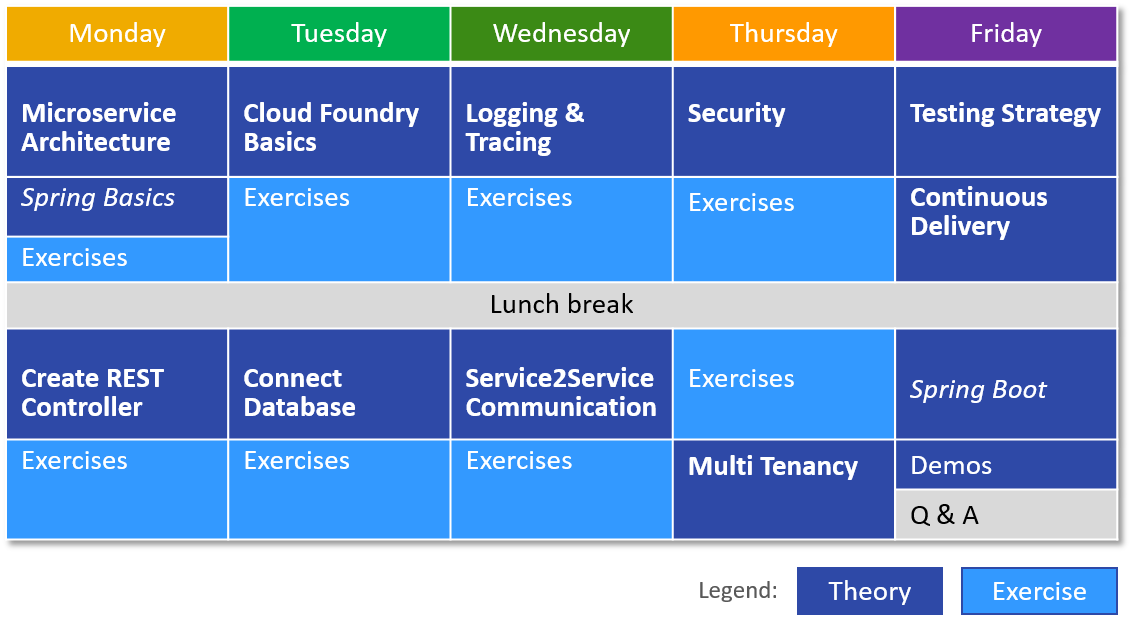
\includegraphics[width=0.9\textwidth]{../Abstract/images/Java_CoursePlan_Simple}
\vfill
\colorlink{https://github.wdf.sap.corp/cc-java-dev/cc-coursematerial/blob/master/AnnouncementOfNewVersion.md}{Announcement of new course Version}
\end{frame}

\begin{frame}{Tips and Tricks - DOs}
\small
\textbf{Maven dependencies (pom.xml)}
\begin{itemize}
\item \ldots add dependencies to the end to avoid overriding defined versions.
\item \ldots add \codealt{<scope>test</scope>} for dependencies required in tests only.
\item \ldots add \codealt{<scope>provided</scope>} for dependencies provided by the CF buildpack.
\item \ldots declare versions explicitly (also true for buildpack version).
\end{itemize}
\textbf{Test code \& test resources}
\begin{itemize}
\item \ldots put test resources into \emph{src/test/java} source folder.
\end{itemize}
\textbf{Configuration defaults}
\begin{itemize}
\item \ldots define defaults e.g. for configuration, which are "valid" in production.
\end{itemize}
\end{frame}

\begin{frame}{Tips and Tricks - DOs}{Continued \ldots}
\small
\textbf{Version control}
\begin{itemize}
\item \ldots add build artefacts such as \emph{war}, \emph{jar} files or \emph{node\_modules} folders to \emph{.gitignore}.
\end{itemize}
\textbf{Personalize central files}
\begin{itemize}
\item \ldots create a "private" copy of central configuration / deployment files such as \emph{manifest.yml} or \emph{logback.xml} to adapt it to your personal needs. 
\end{itemize}
\vfill
\end{frame}
